\documentclass[a4paper, 11pt]{article}

\usepackage[%
backend=biber,
sorting=none,
natbib=true,
style=numeric,
autocite=inline
]{biblatex}
\addbibresource{references.bib}

\defbibenvironment{sources}
{\list
	{}
	{\setlength{\leftmargin}{\bibhang}%
		\setlength{\itemindent}{-\leftmargin}%
		\setlength{\itemsep}{\bibitemsep}%
		\setlength{\parsep}{\bibparsep}}}
{\endlist}
{\item}

\usepackage{fancyhdr}
\pagestyle{fancy}
\fancyhf{}
\renewcommand{\sectionmark}[1]{\markboth{#1}{}}
\fancyhead[ER]{\rightmark}
\fancyhead[OL]{\nouppercase{\leftmark}}
\cfoot{\thepage}

\usepackage{float}
\newfloat{lstfloat}{htb}{lop}

\usepackage[ngerman]{isodate, babel}

\usepackage{lmodern}

\usepackage{hyperref}
\addto\extrasngerman{
	\renewcommand{\sectionautorefname}{Kapitel}
	\renewcommand{\subsectionautorefname}{Abschnitt}
	\renewcommand{\subsubsectionautorefname}{Unterabschnitt}
}

\usepackage{graphicx}
\usepackage{caption}
\captionsetup[figure]{width=10cm}

\usepackage{ragged2e}

\usepackage[T1]{fontenc}
\usepackage[utf8]{inputenc}

\overfullrule=1mm

%opening
\title{Dokumentation zur Projektarbeit digitale Kaffeekasse}
\author{Jan Müller}
\date{\today}

\begin{document}

\maketitle

\section{Einleitung}
\label{sec:intro}
Die Entwicklung von Android Apps zeichnet sich unter anderem dadurch aus, dass die \textit{API Level}\footnote{Zum Zeitpunkt dieser Ausarbeitung existieren 29 API Level.} des \textit{Android Frameworks} unterschiedliche Funktionalitäten bereitstellen.
Die Nutzerverteilung erstreckt sich über mehrere Versionen \autocite{androidhistory}.
Zur Maximierung der potenziellen Nutzer ist es entsprechend notwendig auch ältere API Level zu unterstützen.
Damit Entwickler dort ebenfalls neue Funktionen verwenden können, wurden die \textit{Support Libraries} eingeführt \autocite{supportlibraries}.
Aus diesen entwickelten sich die \textit{Android Jetpack} Bibliotheken \autocite{androidjetpack}.

Ziel dieses Projektes war die Entwicklung einer Kaffeekassen App und einer dazugehörigen Serveranwendung mit der Programmiersprache Kotlin.
Für die Entwicklung der App sollten Android Jetpack Bibliotheken verwendet werden, um ihre Vorzüge und Eigenschaften kennenzulernen.

Diese Dokumentation stellt Architektur, verwendete Bibliotheken und Eigenschaften der digitalen Kaffeekassen App sowie des zugehörigen Servers vor.
Anschließend wird der Entstehungsprozess beider Programme erläutert und ein Fazit zu Android Jetpack gezogen.
%------------------------------------------------------------------------------------------------------------------------------------------------------

\section{Android App}
\label{sec:app}
Kern dieser Projektarbeit ist die Android App, die als Benutzeroberfläche der digitalen Kaffeekasse dient.
Sie basiert auf Grundlagen, welche durch Android Jetpack gelegt wurden.
In diesem Kapitel werden Architektur, verwendete Android Jetpack Komponenten und Bibliotheken sowie Konfiguration der App vorgestellt.
%------------------------------------------------------------------------------------------------------------------------------------------------------

\subsection{Architektur}
\label{subsec:app:architecture}
Die App verwendet die von Google empfohlene \textit{Model-View-ViewModel} Architektur (\textit{MVVM}) \autocite{androidarchitecture}.
Bei dieser wird die Anwendung in Datenmodell, Benutzeroberfläche und die sogenannten \textit{ViewModels} aufgeteilt (siehe \autoref{fig:app:architecture:mvvm}).

Die Ebene des Datenmodells liegt in Form von \textit{Repositories} vor.
Diese kommunizieren über eine Netzwerkschnittstelle mit der Serveranwendung um Daten zu laden oder Aktionen wie Käufe und Logins durchzuführen.
So erhaltene Daten werden unmittelbar in die lokale Datenbank geschrieben und auch nur von dort aus geladen.
Über diesen Mechanismus wird eine lokale Persistenz ermöglicht, wodurch Daten auch ohne Verbindung zum Server angezeigt werden können.
Weil der Zustand eines Datenmodells ausschließlich vom zugehörigen Repository bestimmt wird, werden sie auch als \textit{Single source of truth} bezeichnet.
Durch diese Eigenschaft ist es möglich inkonsistente Datenbestände zu verhindern.

ViewModels passen von Repositories bereitgestellte Daten für Benutzeroberflächen an und stellen sie in Datencontainern bereit.
Sie selbst haben keine Informationen über Benutzeroberflächen.
Stattdessen reagieren diese auf Änderungen an ViewModels und entscheiden selbst über die Datenanzeige.

\begin{figure}[H]
	\centering
	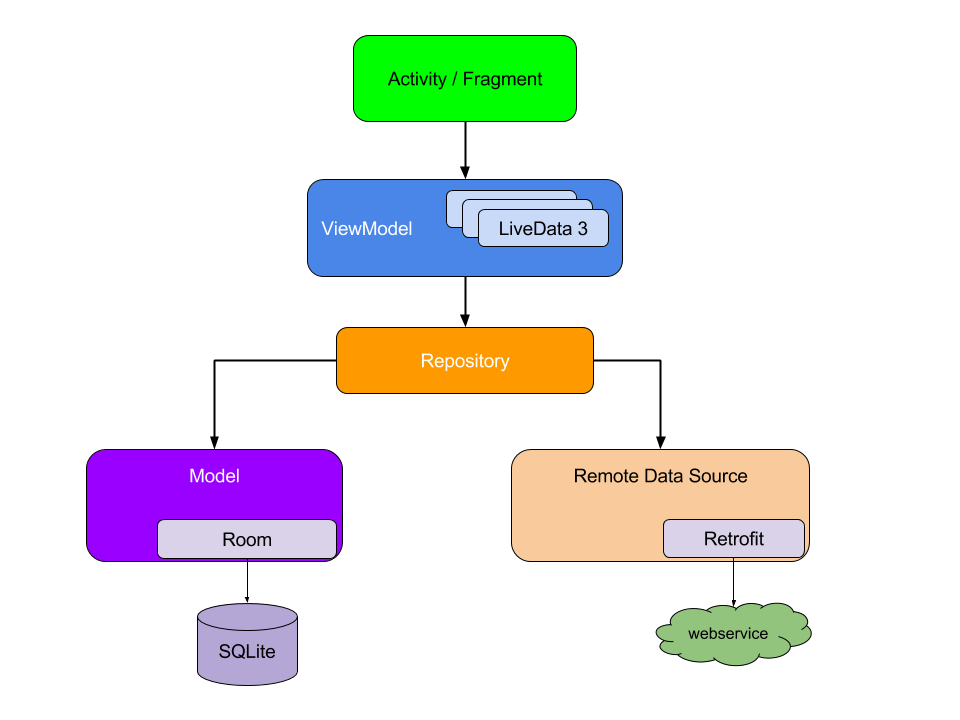
\includegraphics[height=8cm,keepaspectratio]{./images/android-architecture.png}
	\caption{MVVM-Entwurfsmuster in Android}
	\caption*{\small Quelle: \url{https://developer.android.com/topic/libraries/architecture/images/final-architecture.png}}
	\label{fig:app:architecture:mvvm}
\end{figure}
%------------------------------------------------------------------------------------------------------------------------------------------------------

\subsection{Android Jetpack}
\label{subsec:app:jetpack}
Im Folgenden werden die verwendeten Android Jetpack Bibliotheken kurz vorgestellt. Detaillierte Informationen können der offiziellen Dokumentation entnommen werden.
%------------------------------------------------------------------------------------------------------------------------------------------------------

\subsubsection{Core und AppCompat}
\label{subsubsec:app:jetpack:base}
Die \textit{Core} und \textit{AppCompat} Bibliotheken ermöglichen eine Verwendung von Funktionen neuer Android API Levels auf älteren Android Versionen.
Dazu stellen sie eine Vielzahl an Hilfsklassen zur Verfügung, welche die unterschiedliche Behandlung der API Levels verkapseln und die Entwicklung so vereinheitlichen und vereinfachen.
%------------------------------------------------------------------------------------------------------------------------------------------------------

\subsubsection{Fragment}
\label{subsubsec:app:jetpack:fragment}
Fragmente sind modulare Teile einer Benutzeroberfläche.
Sie sind wiederverwendbar, leichtgewichtig und lassen sich in \textit{Activities} sowie anderen Fragmenten kombinieren um komplexe Benutzeroberflächen zu erstellen.
Ihr Lebenszyklus wird von ihrem Container verwaltet, weshalb sie sich für Entwickler nur gering von Activities unterscheiden.
Darüber hinaus ist es möglich Fragmente dynamisch hinzuzufügen und zu entfernen.
Komplexe \textit{Layouts} lassen sich so in mehrere Fragmente unterteilen, welche unabhängig voneinander wiederverwendbar sind.
%------------------------------------------------------------------------------------------------------------------------------------------------------

\subsubsection{Databinding}
\label{subsubsec:app:jetpack:databinding}
Mit Hilfe der \textit{Databinding} Bibliothek ist es möglich Datenquellen für Eigenschaften von Benutzeroberflächen und deren Elemente in Layout-Dateien festzulegen.
In Kombination mit \textit{LiveData} passen sich Benutzeroberflächen bei Änderungen automatisch an, wodurch der Anteil an Quelltext für Benutzeroberflächen reduziert wird.
Zusätzlich lassen sich \textit{BindingAdapters} definieren, durch welche benutzerdefiniertes Verhalten und eine Definition neuer Eigenschaften möglich wird.
%------------------------------------------------------------------------------------------------------------------------------------------------------

\subsubsection{Lifecycle}
\label{subsubsec:app:jetpack:lifecycle}
Die \textit{Lifecycle} Bibliothek umfasst primär ViewModels und LiveData.
Jetpack ViewModels werden vom Android Framework verwaltet und passen sich dem Lebenszyklus des besitzenden Fragments an.

LiveData baut auf diesem Konzept auf.
Dabei handelt es sich um \textit{Wrapper} für beliebige Daten, deren Werte beobachtet werden können.
Anders als traditionelle \textit{Observables} besitzt LiveData jedoch einen Lebenszyklus.
Änderungen werden nur dann propagiert, wenn sie auch beobachtet werden.
Zudem übernimmt das besitzende ViewModel die Verwaltung ihres Lebenszyklus, wodurch \textit{Memory Leaks} vermieden werden.
%------------------------------------------------------------------------------------------------------------------------------------------------------

\subsubsection{Navigation}
\label{subsubsec:app:jetpack:navigation}
Fragmente können mit Argumenten erzeugt werden.
Dabei ist jedoch keine Typsicherheit garantiert und es gibt keinen Mechanismus, der die Vollständigkeit von Argumenten sicherstellt.
Die \textit{Navigation} Bibliothek löst beide Probleme durch Verwendung von Navigationsgraphen.
In diesen werden verfügbare Fragmente und ihre Argumente definiert.
Durch Verbindungen zwischen Fragmenten werden \textit{Directions} angegeben.
Deren Verwendung bei der Navigation stellt sicher, dass alle Argumente mit korrektem Typ vorhanden sind und zum korrekten Fragment navigiert wird.
Darüber hinaus unterstützt die Bibliothek Navigationscontroller, die das Initialisieren von Benutzerelementen wie \textit{Bottom Navigations} und \textit{Hamburger Menus} übernehmen. 
%------------------------------------------------------------------------------------------------------------------------------------------------------

\subsubsection{ConstraintLayout und SwiperefreshLayout}
\label{subsubsec:app:jetpack:layouts}
Android Jetpack umfasst auch mehrere Layout Bibliotheken.
Im Rahmen dieses Projektes wurden \textit{ConstraintLayout} und \textit{SwiperefreshLayout} verwendet.

Komplexe Hierarchien in Benutzeroberflächen verringern deren Performanz bei Layoutänderungen.
ConstraintLayouts ermöglichen das freie Platzieren von Elementen durch Angaben zur Einschränkung ihrer Positionen.
So können Entwickler simplere und effizientere Layouts implementieren.

Bei mobilen Anwendungen gibt es die gängige Geste des Herunterziehens zum Aktualisieren eines Bildschirms.
Mit Hilfe von SwiperefreshLayout ist es möglich diese Funktionalität mit wenigen Zeilen Quelltext zu bestehenden Benutzeroberflächen hinzuzufügen.
%------------------------------------------------------------------------------------------------------------------------------------------------------

\subsubsection{RecyclerView}
\label{subsubsec:app:jetpack:recyclerview}
\textit{RecyclerViews} ermöglichen das Anzeigen von scrollbaren, dynamischen Listen.
Anders als primitive \textit{Views} erzeugt RecyclerView nur tatsächlich benötigten Container und verwendet diese wieder.
Dadurch sind RecyclerViews performanter als beispielsweise \textit{ListViews} oder \textit{LinearLayouts}.
Entwickler müssen Adapter verwenden um Daten an eine RecyclerView zu übergeben.
Es stehen jedoch Hilfsklassen bereit, die bereits über einen Großteil der benötigten Logik verfügen.
%------------------------------------------------------------------------------------------------------------------------------------------------------

\subsubsection{Room}
\label{subsubsec:app:jetpack:room}
Bei \textit{Room} handelt es sich um eine Abstraktionsebene für \textit{SQLite} Datenbanken.
Es können sowohl programmatische als auch reguläre SQL Anfragen definiert werden.
Die Hauptfunktion von Room liegt jedoch in der Möglichkeit Rückgabewerte in reaktiven Wrapper-Klassen, wie beispielsweise LiveData, zu erhalten.
Room übernimmt in diesem Fall die Aktualisierung der Daten, wodurch es reicht Datenbankanfragen einmalig auszuführen.
%------------------------------------------------------------------------------------------------------------------------------------------------------

\subsubsection{Paging}
\label{subsubsec:app:jetpack:paging}
Das Laden großer Datenmengen aus Datenbanken oder Netzwerkquellen ist ein nicht zu unterschätzender Aufwand.
Die \textit{Paging} Bibliothek ermöglicht deshalb ein stückweises Laden von Datensätzen.
Dazu muss eine \textit{DataSource Factory} vorliegen, welche dieses Konzept unterstützt.
Unter anderem ermöglicht Room solche Factories als Rückgabewerte zu definieren.
Sie lassen sich zu LiveData Objekten transformieren, welche \textit{PagedLists} enthalten.
Diese besonderen Listen lassen sich unter anderem mit RecyclerViews und \textit{PagedListAdaptern} verwenden.
Im Endeffekt können so Performanz und Speicherverbrauch verbessert werden.
%------------------------------------------------------------------------------------------------------------------------------------------------------

\subsubsection{Work}
\label{subsubsec:app:jetpack:work}
Hintergrundaufgaben, wie beispielsweise das Bereinigen von Datenbanken, können über die \textit{Work} Bibliothek verwaltet werden.
Die zu erledigende Arbeit wird dabei in einer \textit{Worker} Klasse definiert.
Bei der Registrierung können optional Einschränkungen angegeben werden, die festlegen wann und unter welchen Umständen der Worker ausgeführt wird.
%------------------------------------------------------------------------------------------------------------------------------------------------------

\subsubsection{KTX}
\label{subsubsec:app:jetpack:extensions}
Kotlin ist die von Google empfohlene Sprache für die Entwicklung von Android Apps \autocite{androidkotlin}.
Eine Vielzahl an Android Jetpack Bibliotheken enthalten Erweiterungsmethoden und Sprachfunktionen, welche die Programmierung von Android Apps mit Kotlin vereinfachen und verbessern.
Dazu zählen unter anderem Methoden zum Erzeugen von ViewModels sowie \textit{Coroutine Scopes} für ViewModels, Erweiterungen für \textit{SharedPreferences} und Unterstützung für \textit{Coroutines} in Android Jetpack Bibliotheken.
%------------------------------------------------------------------------------------------------------------------------------------------------------

\subsection{Weitere Bibliotheken}
\label{subsec:app:bibs}
Im Rahmen der App-Entwicklung wurden auch Bibliotheken verwendet, welche nicht Teil von Android Jetpack sind.
Im Folgenden werden ihre Funktionen und Verwendungsgründe vorgestellt.
%------------------------------------------------------------------------------------------------------------------------------------------------------

\subsubsection{Retrofit und Moshi}
\label{subsubsec:app:bibs:retrofitmoshi}
Über \textit{Retrofit} können abstrakte Methoden zum Anbinden von APIs definiert werden.
Entwickler müssen dazu Informationen über die Art von Anfragen angeben.
Implementierungen dieser Methoden werden von der Bibliothek generiert.
In Kombination mit der Serialisierungs-Bibliothek \textit{Moshi} können so Netzwerkschnittstellen mit geringem Quelltextaufwand angebunden werden.
%------------------------------------------------------------------------------------------------------------------------------------------------------

\subsubsection{Glide}
\label{subsubsec:app:bibs:glide}
\textit{Glide} übernimmt das asynchrone Laden und Darstellen von Bildern.
Dabei lassen sich Einstellungen für Verhalten und Darstellung anpassen.
Unter anderem kann Glide Bilder für schnelleres Laden zwischenspeichern, zuschneiden und während einem Ladevorgang durch Platzhalter ersetzen.
%------------------------------------------------------------------------------------------------------------------------------------------------------

\subsubsection{Image Picker}
\label{subsubsec:app:bibs:imagepicker}
Die Bibliothek \textit{Image Picker} ermöglicht die Auswahl von Bildern zur Laufzeit, die Nutzer entweder aus ihrer Galerie auswählen oder mit ihrer Kamera aufnehmen können.
Eine äquivalente Funktionalität zu implementieren ist mit nicht-trivialem Aufwand verbunden, weshalb eine Verwendung existierender Bibliotheken die Entwicklung verkürzte.
%------------------------------------------------------------------------------------------------------------------------------------------------------

\subsubsection{PrettyTime}
\label{subsubsec:app:bibs:prettytime}
\textit{PrettyTime} wird verwendet um Zeitstempel in ein für Menschen lesbares Format zu transformieren.
Die Bibliothek unterstützt mehrere Sprachen, unter anderem Deutsch sowie Englisch, und erspart Entwicklern so das Übersetzen und Formatieren.
%------------------------------------------------------------------------------------------------------------------------------------------------------

\subsubsection{Timber}
\label{subsubsec:app:bibs:timber}
Bei \textit{Timber} handelt es sich um eine Bibliothek die das Protokollieren vereinfacht, Nachrichten mit zusätzlichen Informationen wie beispielsweise ihrem Ursprung ausgibt und jegliche Protokollierung außerhalb der Entwicklungsphase deaktiviert.
So ist es während der Entwicklung möglich schnell detaillierte Protokollnachrichten zu verfassen, welche bei der Suche nach Fehlern helfen und keine Auswirkung auf ausgelieferte Endprodukte haben.
%------------------------------------------------------------------------------------------------------------------------------------------------------

\subsection{Konfiguration}
\label{subsec:app:configuration}
Zur Konfiguration muss die Adresse der Serveranwendung angepasst werden.
Dies findet über den Wert des Feldes \verb|KOFFEE_BACKEND_URL|, in der Datei \verb|build.gradle|, statt.
Eine weitere Konfiguration ist nicht notwendig.
%------------------------------------------------------------------------------------------------------------------------------------------------------

\section{Serveranwendung}
\label{sec:backend}
Das Backend wurde, wie auch die App, mit der Programmiersprache Kotlin entwickelt.
Es handelt sich dabei um eine \textit{REST}-Schnittstelle\footnote{Siehe \url{https://restfulapi.net/}.}, die dazu dient den Zustand der digitalen Kaffeekasse zu verwalten.
Die folgenden Abschnitte stellen Architektur, Authentifizierung, verwendete Bibliotheken sowie Konfiguration und Inbetriebnahme des Backends vor.
%------------------------------------------------------------------------------------------------------------------------------------------------------ 

\subsection{Architektur}
\label{subsec:backend:architecture}
Das Backend verwendet eine serviceorientierte Architektur.
Dabei werden Anfragen an Dienste weitergeleitet.
Antworten von Diensten enthalten Informationen über die Ergebnisse von Aktionen, wie Statuscodes, Daten oder Fehlermeldungen, und werden an Kommunikationspartner weitergeleitet.

Es existieren Dienste für Nutzer-, Profilbild-, Artikel- und Transaktionsverwaltung.
Validierung sowie Fehlerbehandlung finden ausschließlich in Diensten statt.
Dafür verwenden sie einen funktionalen Ansatz und sind selbst zustandslos.

Analog zur Android App liegt die Persistenzebene in Form von Repositories vor.
Die gegebenen Implementierungen der Nutzer-, Profilbild- und Artikel-Repositories fungieren als Schnittstellen zur verwendeten \textit{MongoDB}.

Sowohl Dienste als auch Repositories liegen als \textit{Interfaces} und Implementierungen vor, um separates Testen zu ermöglichen.
%------------------------------------------------------------------------------------------------------------------------------------------------------

\subsection{Authentifizierung}
\label{subsec:backend:authentication}
Um Administrator-Funktionen zu verwenden müssen sich Nutzer authentifizieren.
Dies findet mit Hilfe von \textit{JSON Web Tokens}\footnote{Siehe \url{https://jwt.io/}.}, auch \textit{JWT} genannt, statt.
Ein JWT wird nach einem erfolgreichen Login generiert, ist für 24 Stunden gültig und muss bei jeder Anfrage für Administrator-Funktionen enthalten sein.
Einloggen können sich nur Nutzer, die über Administratorrechte verfügen, welche wiederum nur von Administratoren vergeben werden können.
Während jedem Start generiert das Backend einen Standard\-administrator, welcher zuvor festgelegte Daten besitzt (siehe \autoref{subsec:backend:configuration}).
%------------------------------------------------------------------------------------------------------------------------------------------------------

\subsection{Bibliotheken}
\label{subsec:backend:bibs}
Um die Entwicklung des Backends zu beschleunigen wurden mehrere Open Source Bibliotheken verwendet.
Diese werden im Folgenden kurz vorgestellt.
Zusätzliche Informationen können den jeweiligen Projektseiten entnommen werden.
%------------------------------------------------------------------------------------------------------------------------------------------------------

\subsubsection{Ktor}
\label{subsubsec:backend:bibs:ktor}
\textit{Ktor}, ein \textit{Web Framework} vom Entwickler der Sprache Kotlin, bildet die Grundlage des Backends.
Ktor verwendet eine \textit{Domain Specific Language}, auch \textit{DSL} genannt, zum Definieren von Modulen.
Solche Module können in der Serveranwendung installiert werden um ein erwünschtes Verhalten zu erreichen.
Ktor selbst stellt dabei Module für verschiedene Bereiche, wie unter anderem Protokollierung, Serialisierung und Authentifizierung, zur Verfügung.
Auch vordefinierte Module können im Quelltext angepasst werden.
Ktor zeichnet sich zudem dadurch aus, dass es vollständig asynchron arbeitet und Kotlin Coroutines an allen Stellen der Konfiguration verwendbar sind.
Dadurch können Entwickler asynchronen und performanten Quelltext schreiben, ohne zusätzliche Sprachkonstrukte zu verwenden.
%------------------------------------------------------------------------------------------------------------------------------------------------------

\subsubsection{Koin}
\label{subsubsec:backend:bibs:koin}
\textit{Koin} ist ein Framework für \textit{Dependency Injection}, mit dem einzelne Komponenten des Servers unabhängig von ihrem Einsatzort initialisiert werden können.
So ist es möglich Instanzen von Diensten sowie Repositories wiederzuverwenden und den für Instanziierung benötigten Quelltext zu minimieren.
%------------------------------------------------------------------------------------------------------------------------------------------------------

\subsubsection{KMongo}
\label{subsubsec:backend:bibs:kmongo}
Die \textit{KMongo} Bibliothek ermöglicht eine simple Verwendung von \textit{Mongo}-Datenbanken in Kotlin.
Dies erreicht sie durch automatische Serialisierung, Unterstütztung für Kotlin Coroutines und programmatische, typsichere Anfragen.
%------------------------------------------------------------------------------------------------------------------------------------------------------

\subsubsection{jBCrypt}
\label{subsubsec:backend:bibs:jbcrypt}
Das Backend muss Passwörter sicher in der Datenbank ablegen.
Dafür müssen diese mit einer geeigneten \textit{Hash}-Funktion transformiert werden.
Die Bibliothek \textit{jBCrypt} enthält solche Funktionen.
Darüber hinaus ermöglicht sie auch das anschließende Überprüfen von Passwörtern.
%------------------------------------------------------------------------------------------------------------------------------------------------------

\subsubsection{Arkenv}
\label{subsubsec:backend:bibs:arkenv}
Zur Konfiguration des Backends an eine Einsatzumgebung müssen einige Parameter, wie die Adresse der Datenbank, gesetzt werden.
\textit{Arkenv} erlaubt es diese Umgebungsvariablen programmatisch und typsicher zu definieren, so dass die Fehleranfälligkeit beim Einlesen reduziert wird.
%------------------------------------------------------------------------------------------------------------------------------------------------------

\subsubsection{Docker Secrets}
\label{subsubsec:backend:bibs:dockersecrets}
Neben Umgebungsvariablen müssen auch sensible Daten, wie die Zugangsinformationen des Standardadministrators, festgelegt werden.
Um diese zu schützen werden beim \textit{Deployment} des Backends mit Docker sogenannte \textit{Secrets} verwendet, welche nur das Backend selbst einsehen kann.
Da es sich dabei um Dateien handelt ist das Einlesen ihrer Informationen mit einer Syntaxanalyse verbunden.
Die leichtgewichtige Bibliothek \textit{Docker Secrets} übernimmt diesen Aufwand und lädt Parameter von Dateien in \textit{Maps}.
%------------------------------------------------------------------------------------------------------------------------------------------------------

\subsection{Konfiguration und Inbetriebnahme}
\label{subsec:backend:configuration}
Um das Backend an Einsatzumgebungen anzupassen sollten einige Parameter konfiguriert werden.
Dies findet über \verb|.env|-Dateien statt, welche sich in dem \verb|environments|-Ordner des Hauptverzeichnisses befinden.
Dort werden die Adressen von Server und Datenbank sowie Eigenschaften der Zertifizierung festgelegt.
Darüber hinaus werden die Namen der Docker Secrets-Dateien angegeben, in welchen sensible Daten hinterlegt werden.
Bei der Standardkonfiguration müssen sich diese im \verb|secrets|-Verzeichnis befinden.
\verb|hmac_secret.secret| enthält den zur Signierung von JWTs verwendeten Schlüssel.
Dabei kann es sich um eine beliebige Zeichenkette handeln.
Analog zur Syntax von \verb|.env|-Dateien muss \verb|default_admin.secret| die Werte \verb|ID|, \verb|NAME| und \verb|PASSWORD| enthalten, welche zur Erzeugung von Standardadministratoren verwendet werden.

Um das Backend in Betrieb müssen zuerst der \verb|URL|-Parameter in der Datei \verb|domain.env| angepasst und beide \verb|.secret|-Dateien angelegt werden.
Nachdem das Projekt mit dem Befehl \verb|./gradlew build| erzeugt wurde, kann die Serveranwendung über Docker Compose gestartet werden.
Detaillierte Informationen zur Syntax dieser Konfigurationsdateien sowie Inbetriebnahme und Wartung des Backends können der \verb|README.md|-Datei entnommen werden, welche dem Projekt beiliegt und dieser Dokumentation anhängt.
%------------------------------------------------------------------------------------------------------------------------------------------------------

\section{Vorgehen und Entstehungsprozess}
\label{sec:methodologies}
Die Projektarbeit begann mit der Entwicklung des Backends.
Zunächst wurden Aufbau sowie Struktur festgelegt und implementiert um eine Arbeitsgrundlage zu schaffen.
Dank der modularen Zusammensetzung des Backends war es möglich die benötigten Endpunkte für Nutzer, Artikel sowie Transaktionen schnell und unabhängig voneinander zu implementieren.
Anschließend wurde die Authentifizierung hinzugefügt um Endpunkte vor unautorisierten Zugriffen zu schützen.
Da eine langfristige Nutzung des Backends in Frage kam, wurde der Quelltext nahezu vollständig getestet.
Tests wurden parallel zum eigentlich Programm geschrieben um Fehler schnell zu erkennen.
Im Laufe der Entwicklung wurde das Backend mehrfach überarbeitet um einen möglichst funktionalen Programmierstil zu erreichen.
So konnten Lesbarkeit des Quelltextes verbessert und Fehleranfälligkeit reduziert werden.
Während der gesamten Projektarbeit wurde zudem die Formatierung des Quelltextes mit dem Tool \textit{klint}\footnote{Siehe \url{https://github.com/pinterest/ktlint}.} kontrolliert und korrigiert.
Darüber hinaus wurden Open Source Bibliotheken verwendet, falls Problemlösungen einen größeren Aufwand erforderten.
Dadurch konnte die Entwicklungszeit verkürzt und auf die eigentliche Aufgabenstellung fokussiert werden.

Die Entwicklung der App begann Ende April.
Analog zu den Endpunkten des Backends wurden die Bildschirme der App nacheinander implementiert, wobei jeweils mehrere Revisionen durchgeführt wurden.
Eine Verwendung der Android Jetpack Bibliotheken erlaubten dabei eine schnelle Entwicklung mit einem geringen Anteil an Boilerplate Code.
Um diesen weiter zu reduzieren wurden im Laufe der Entwicklung häufig auftretende Muster, wie beispielsweise von ViewModels initiierte Aktionen, in Klassen ausgelagert.
Auch bei den ViewModels selbst sowie Fragmenten wurde Vererbung verwendet um oft benötigtes Verhalten nicht mehrfach zu implementieren.
Zudem wurde die Fehlerbehandlung zentralisiert um die Fehlerausgabe zu vereinfachen und Abstürze zu verhindern.
Durch solche Änderungen war es möglich den Quelltext deutlich zu kürzen.

Zunächst wurde die App für einen Nutzer pro Endgerät entwickelt.
Anfang Juni wurde, nach Anfrage des Projektbetreuers, ein zusätzlicher Modus für mehrere Nutzer implementiert.
Weil die einzelnen Komponenten der App bereits modular und wiederverwendbar waren, konnte diese größere Änderung schnell umgesetzt werden. 
Im Anschluss wurden ein Großteil der Benutzeroberflächen sowie deren Verwendung überarbeitet und verbessert.

Nachdem die Funktionalität beider Teilprojekte vollständig implementiert war, wurde mit der Dokumentation des Quelltextes begonnen, welche im Internet abrufbar ist\footnote{Siehe \url{http://koffee-app.yeger.eu/} und \url{http://koffee-backend.yeger.eu/}.}.
%------------------------------------------------------------------------------------------------------------------------------------------------------

\section{Ergebnisse}
\label{sec:results}
%------------------------------------------------------------------------------------------------------------------------------------------------------

\section{Fazit}
\label{sec:conclusion}
Die Vorzüge der Android Jetpack Bibliotheken zeigten sich bereits während der Entwicklung.
Mit Fragmenten und ViewModels war es möglich neue Bildschirme schnell zu implementieren.
Zudem ermöglichten Android Jetpacks visuelle Navigationsgraphen ein einfaches und übersichtliches Verknüpfen von Fragmenten.
Der dadurch gewonnene Gesamtüberblick resultierte in einer sicheren und fehlerresistenten Struktur.
Der automatisierte Lebenszyklus vieler Jetpack Komponenten erlaubte zudem eine Minimierung an Interaktionen mit dem Android Framework.
Stattdessen war es möglich den Fokus auf das Verhalten von Benutzeroberflächen und Geschäftslogik zu legen.
Des Weiteren hat sich Room als eine der wichtigsten Komponenten von Android Jetpack erwiesen.
Bei der Entwicklung trivialisierte sie Datenbankzugriffe und reduzierte Datenverwaltung auf ein Minimum.
Sichtbar wurden diese Vorzüge besonders bei der Entwicklungszeit.
Meilensteine wurden meist Wochen zuvor erreicht, wodurch zusätzliche Funktionen implementiert werden konnten.

Auch bei Verwendung der App sind Vorzüge der Jetpack Bibliotheken erkennbar.
Die Asynchronität der Kombination von Room, LiveData und ViewModels stellt sicher, dass Datenbankzugriffe nicht zu einer Blockierung der Benutzeroberfläche führen.
RecyclerViews sorgen zudem für eine performante Darstellung von Listen und ermöglichen flüssiges Scrollen durch diese.
Die Paging Bibliothek begünstigt dies weiter.
Sie sorgt dafür, dass das Laden von Listen aus der Datenbank auch bei vielen Einträgen nicht langsamer wird.
Lifecycle Komponenten sorgen zudem dafür, dass sie nicht länger als benötigt aktiv bleiben, wodurch Speicher- sowie Prozessorverbrauch reduziert werden.

Mit Android Jetpack Bibliotheken entwickelte Apps sind zwar nicht zwingend schneller oder besser als Herkömmliche, jedoch ist es für Entwickler einfacher diese Ziele zu erreichen, da Grundbausteine und Architektur bereits gegeben sind.
Weil sie zugleich eine beschleunigte Entwicklung ermöglichen und die Zukunft der von Google entwickelten Android Bibliotheken bilden, ist es empfehlenswert bei der App Entwicklung auf Jetpack Komponenten zurückzugreifen.
%------------------------------------------------------------------------------------------------------------------------------------------------------

\newpage
\begingroup
\raggedright
\printbibliography[title={Referenzen}, keyword=citations]
\nocite{*}
\newrefcontext[sorting=nty]
\printbibliography[title={Dokumentation}, keyword=sources, env=sources]
\endgroup

\end{document}
